\documentclass[11pt,a4paper]{article}

% --- Packages ---------------------------------------------------------------
\usepackage[utf8]{inputenc}
\usepackage[T1]{fontenc}
\usepackage{lmodern}
\usepackage[margin=2.5cm]{geometry}
\usepackage{amsmath,amssymb}
\usepackage{graphicx}
\usepackage{booktabs}
\usepackage{enumitem}
\usepackage{xcolor}
\usepackage{listings}
\usepackage{tikz}
\usetikzlibrary{arrows.meta,positioning,shapes.geometric,fit,calc}
\usepackage{float}
\usepackage{caption}
\usepackage{parskip}
\usepackage[most]{tcolorbox}
\usepackage{titlesec}
\usepackage{hyperref}

% --- Color palette ----------------------------------------------------------
\definecolor{primary}{RGB}{30,72,120}
\definecolor{accent}{RGB}{180,80,40}
\definecolor{softgray}{RGB}{96,96,96}
\definecolor{boxbg}{RGB}{245,248,252}
\definecolor{boxborder}{RGB}{30,72,120}

\hypersetup{
  colorlinks=true,
  linkcolor=primary,
  citecolor=primary,
  urlcolor=accent,
}

% --- Section styling --------------------------------------------------------
\titleformat{\section}
  {\color{primary}\Large\bfseries\sffamily}
  {\thesection}{0.6em}{}
  [\vspace{2pt}{\color{primary!40}\titlerule[0.6pt]}]
\titleformat{\subsection}
  {\color{primary!85!black}\large\bfseries\sffamily}
  {\thesubsection}{0.5em}{}
\titleformat{\subsubsection}
  {\color{primary!75!black}\normalsize\bfseries\sffamily}
  {\thesubsubsection}{0.4em}{}

\newtcolorbox{insightbox}[1][]{
  enhanced, breakable,
  colback=boxbg, colframe=boxborder,
  boxrule=0.4pt, arc=2pt,
  left=8pt, right=8pt, top=6pt, bottom=6pt,
  fonttitle=\bfseries\sffamily\color{white},
  coltitle=white,
  colbacktitle=primary,
  attach boxed title to top left={xshift=6pt, yshift=-2mm},
  boxed title style={colback=primary, sharp corners, boxrule=0pt},
  #1
}

\lstset{
  basicstyle=\ttfamily\small,
  keywordstyle=\color{primary}\bfseries,
  commentstyle=\color{green!40!black}\itshape,
  stringstyle=\color{accent},
  breaklines=true,
  frame=single,
  rulecolor=\color{gray!40},
  backgroundcolor=\color{boxbg},
  numbers=left,
  numberstyle=\tiny\color{gray},
  numbersep=6pt,
  language=Python,
  showstringspaces=false,
}

% --- Title -------------------------------------------------------------------
\title{%
  \color{primary}\textbf{Dynamic GraphRAG for Open Scientific Question Answering}\\[0.5em]
  \large\color{softgray} A Graph-Augmented Retrieval System with Confidence-Driven\\
  Adaptive Expansion and Plan-Aware Pipeline Orchestration%
}
\author{Fadel Fatima Zahra \quad Benfellah Ikram \quad Samia Lachgar}
\date{April 2026}

\begin{document}
\maketitle
\thispagestyle{empty}

% --- Abstract ----------------------------------------------------------------
\begin{abstract}
\noindent
We propose \textbf{Dynamic GraphRAG}, a multi-stage retrieval-augmented
generation system designed to answer open-ended scientific questions by
constructing ephemeral knowledge graphs over live academic literature. In
contrast to classical RAG pipelines, which concatenate retrieved passages
into a flat context, and to existing GraphRAG approaches, which depend on
static or partially structured representations, the proposed approach
extracts typed entities and directed relations from paper abstracts,
assembles a per-query directed graph, and retrieves a query-relevant
subgraph through embedding-driven seed selection and multi-hop traversal.
The final answer is generated by conditioning the language model on both
structured graph triples and the originating paper evidence. The pipeline
is domain-agnostic and currently supports queries in Agriculture,
Geoscience, Computer Science, Supply Chain, and Environment without any
domain-specific prompts. A confidence-driven adaptive expansion mechanism
re-retrieves literature and rebuilds the graph whenever coverage validation
fails, bounded to two iterations to control latency. An LLM-based query
planner classifies each question into one of five reasoning archetypes and
emits a structured plan that shapes retrieval weighting, extraction
priorities, validation thresholds, and answer formatting. A four-mode
ablation framework covering 22 benchmark questions evaluates ROUGE, keyword
coverage, semantic similarity, and LLM-as-a-judge scores across
progressively richer configurations, and isolates the contribution of graph
structure, reasoning paths, and adaptive expansion.
\end{abstract}

\tableofcontents
\newpage

% =============================================================================
\section{Introduction}
% =============================================================================

\subsection{Problem Framing: Limitations of Classical RAG and Static GraphRAG}

Retrieval-augmented generation (RAG) has become the standard paradigm for
grounding large language models in external evidence. In its canonical form,
the model retrieves the top-$k$ documents for a query and concatenates them
into a flat prompt~\cite{lewis2020rag}. While this strategy is effective for
narrow factual lookup, it exhibits systematic failure modes on open scientific
questions. Flat context suppresses cross-document structure: if one paper
reports that drought \emph{causes} stomatal closure, and another that stomatal
closure \emph{reduces} photosynthesis, the concatenated prompt does not encode
that causal chain explicitly. Ranking is also performed at the document level
rather than the concept level, so key entities buried in mid-ranked passages
are routinely lost. As a consequence, classical RAG offers no explicit
mechanism for multi-hop reasoning, no structural representation of inter-paper
relationships, and no means of dynamically refining its own retrieval when
evidence is insufficient.

GraphRAG partially addresses these weaknesses by introducing structured
entity-relation representations over the retrieved corpus~\cite{edge2024graphrag}.
However, most deployments rely on \emph{static} or \emph{precomputed} graphs
constructed offline. For open scientific search, this assumption is
restrictive in three respects. First, query intent varies substantially across
definition, comparison, causal analysis, and optimisation, yet a single static
graph cannot encode the entity-type priorities and relation priorities that
each intent demands. Second, static graphs become stale as the underlying
literature evolves, an acute issue in fast-moving scientific fields. Third,
large prebuilt graphs accumulate weak or irrelevant edges whose inclusion
increases retrieval noise rather than reasoning signal. The resulting
pipelines are therefore poorly matched to diverse, intent-sensitive scientific
queries.

\subsection{Research Gap}

The limitations above point to a shared research gap. Existing retrieval
architectures, both flat RAG and classical GraphRAG, lack three capabilities
that are prerequisites for reliable open scientific question answering:

\begin{itemize}[leftmargin=1.2em,itemsep=2pt]
  \item \textbf{Query-specific graph construction.} Knowledge structures are
  assumed to be shared across queries, rather than constructed fresh to
  reflect the entities, relations, and reasoning shape of the question at
  hand.
  \item \textbf{Adaptive reasoning pipelines.} Stage execution is fixed in
  advance, so the system cannot modulate retrieval weighting, extraction
  priorities, or validation thresholds based on the reasoning archetype of
  the query.
  \item \textbf{Confidence-driven retrieval refinement.} Pipelines typically
  execute a single retrieval pass and commit to its output, with no explicit
  mechanism for re-retrieving and re-building the knowledge structure when
  coverage is demonstrably insufficient.
\end{itemize}

\subsection{Positioning Statement}

While existing GraphRAG approaches rely on static or partially structured
representations, our approach introduces a fully dynamic, query-scoped graph
construction pipeline combined with confidence-driven adaptive expansion.
Concretely, each question induces a fresh directed graph assembled at
inference time from live academic literature; retrieval, extraction,
validation, and generation are conditioned on a structured query plan emitted
by an LLM-based planner; and a confidence scorer closes the loop by triggering
targeted re-retrieval whenever the graph fails to satisfy coverage
requirements. The graph is treated not as a persistent artifact, but as a
transient reasoning scaffold assembled on demand and discarded after answer
generation.

\subsection{Contributions}

\noindent Our contributions are:

\begin{itemize}[leftmargin=1.2em,itemsep=3pt]
  \item \textbf{Query-scoped dynamic knowledge graph construction.} The system
  builds a fresh, per-query directed graph from live literature, ensuring that
  the knowledge structure reflects the entities and relations of the current
  question rather than a stale, pre-indexed corpus.
  \item \textbf{Confidence-driven adaptive expansion loop.} A composite
  confidence score combined with a plan-defined coverage validator triggers
  bounded re-retrieval and graph reconstruction whenever evidence is
  insufficient, turning retrieval into a closed-loop process rather than a
  one-shot operation.
  \item \textbf{Plan-aware pipeline orchestration.} An LLM-generated query
  plan classifies the reasoning archetype and propagates to every downstream
  stage, shaping retrieval weighting, entity-extraction priorities,
  validation thresholds, and answer formatting.
  \item \textbf{Robust multi-level fallback strategies.} A three-tier
  extraction cascade, a Groq-to-Ollama rate-limit circuit breaker, and a
  deterministic graph-only answer compiler jointly ensure that the pipeline
  terminates with a grounded answer even under API instability or
  structurally degenerate LLM outputs.
  \item \textbf{Ablation-based evaluation framework.} A four-mode ablation
  study over 22 benchmark questions isolates the contribution of graph
  structure, reasoning paths, and confidence-driven expansion, combining
  lexical, semantic, and LLM-as-a-judge metrics.
\end{itemize}

The remainder of this report describes the system implementing this paradigm
end to end across eight pipeline stages, a session-aware caching layer, and
a confidence-driven expansion loop, all orchestrated through a unified query
plan. Design decisions and engineering tradeoffs that emerged from working
with imperfect external APIs, noisy LLM outputs, and scientific corpora of
variable quality are discussed alongside the architectural presentation.

% =============================================================================
\section{System Overview}
% =============================================================================

The pipeline processes a natural-language scientific question through eight
sequential stages, each implemented as an independent module with explicit,
typed data contracts. No hidden shared state is passed between stages, a
design choice that preserves testability and enables the ablation studies
reported in Section~\ref{sec:evaluation}.

\begin{figure}[H]
\centering
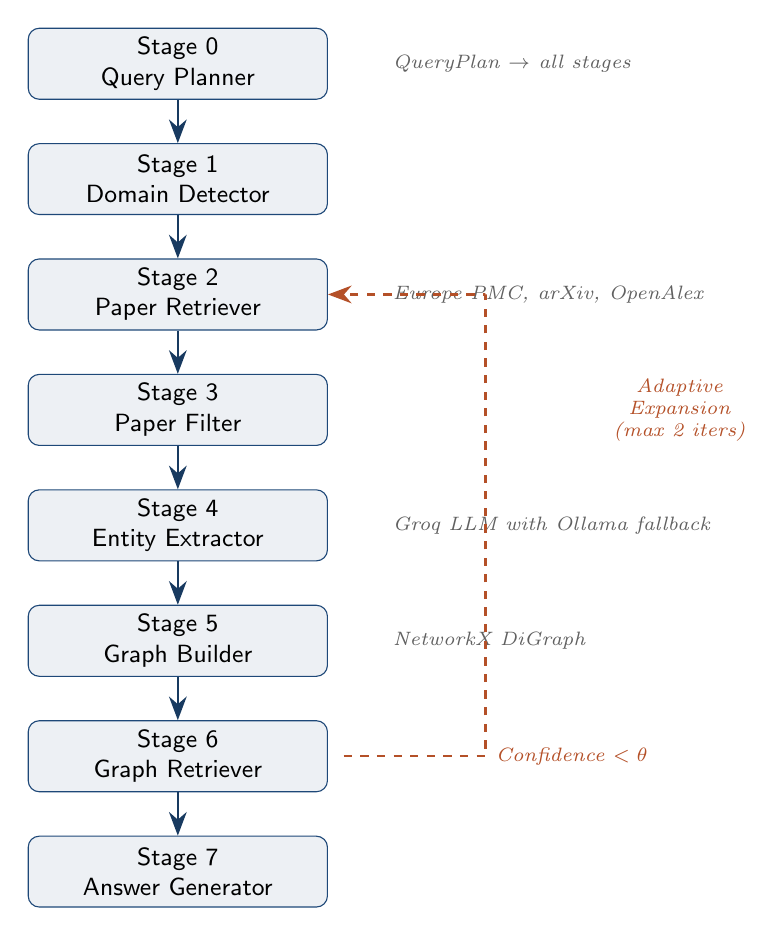
\begin{tikzpicture}[
    stage/.style={
      rectangle, rounded corners=4pt, draw=primary, fill=primary!8,
      minimum width=3.8cm, minimum height=0.9cm, align=center,
      font=\small\sffamily
    },
    arrow/.style={-{Stealth[length=3mm]}, thick, draw=primary!80!black},
    note/.style={font=\scriptsize\itshape, text=softgray, align=center},
    node distance=0.55cm
  ]
  \node[stage]                      (qp)  {Stage 0\\Query Planner};
  \node[stage, below=of qp]        (dd)  {Stage 1\\Domain Detector};
  \node[stage, below=of dd]        (pr)  {Stage 2\\Paper Retriever};
  \node[stage, below=of pr]        (pf)  {Stage 3\\Paper Filter};
  \node[stage, below=of pf]        (ee)  {Stage 4\\Entity Extractor};
  \node[stage, below=of ee]        (gb)  {Stage 5\\Graph Builder};
  \node[stage, below=of gb]        (gr)  {Stage 6\\Graph Retriever};
  \node[stage, below=of gr]        (ag)  {Stage 7\\Answer Generator};

  \draw[arrow] (qp) -- (dd);
  \draw[arrow] (dd) -- (pr);
  \draw[arrow] (pr) -- (pf);
  \draw[arrow] (pf) -- (ee);
  \draw[arrow] (ee) -- (gb);
  \draw[arrow] (gb) -- (gr);
  \draw[arrow] (gr) -- (ag);

  \node[note, right=0.7cm of qp] {QueryPlan $\to$ all stages};
  \node[note, right=0.7cm of pr] {Europe PMC, arXiv, OpenAlex};
  \node[note, right=0.7cm of ee] {Groq LLM with Ollama fallback};
  \node[note, right=0.7cm of gb] {NetworkX DiGraph};

  \draw[arrow, dashed, accent]
    ($(gr.east)+(0.2,0)$) --
    ++(1.8,0) node[note, right, text=accent] {Confidence $< \theta$}
    |- ($(pr.east)+(2.0,0)$) -- (pr.east);

  \node[note, right=3.5cm of pf, text=accent] {Adaptive\\Expansion\\(max 2 iters)};
\end{tikzpicture}
\caption{Dynamic GraphRAG pipeline with confidence-driven adaptive expansion loop.}
\label{fig:pipeline}
\end{figure}

The query plan produced in Stage~0 propagates to every downstream stage,
shaping retrieval weighting (Stage~2), entity extraction priorities
(Stage~4), graph validation thresholds (Stage~6), and answer structure
(Stage~7). When the confidence scorer judges the graph insufficient after
Stage~6, the adaptive expansion loop re-enters at Stage~2 with an enriched
query, merges the new evidence into the existing graph, and re-runs retrieval
and answer generation.

% =============================================================================
\section{Architecture}
% =============================================================================

This section describes each implemented module of the pipeline.

% ---------------------------------------------------------------------------
\subsection{Query Planner}

The Query Planner sits at Stage~0 of the pipeline and classifies each
incoming question into one of five domain-agnostic reasoning types:
definition, comparison, method/process, causal mechanism, or optimization.
Classification is performed by an LLM (Groq backend) that returns a
structured JSON object containing the reasoning type, key entities,
comparison dimensions, intent signals, and an estimated complexity level.

\paragraph{Fallback mechanism.}
When the LLM call fails or produces unparseable output, a heuristic classifier
takes over. It matches the query against curated keyword patterns
(``what is'' $\rightarrow$ definition, ``why'' $\rightarrow$ causal mechanism)
and extracts noun-phrase entities via regular expressions. Every query is
therefore guaranteed a valid plan, regardless of API availability.

\paragraph{Downstream influence.}
The plan drives every subsequent stage through four module-level dictionaries.
Extraction priorities specify which entity types matter most for each
reasoning type (causal questions, for instance, prioritise Cause/Factor and
Effect/Outcome nodes). Relation priorities play the same role for edges.
Answer-structure templates provide format guidance such as
\textit{causal\_chain} for causal questions or \textit{table\_or\_contrast} for
comparisons. Finally, minimum graph requirements record the node, edge, and
type counts that coverage validation will check for.

% ---------------------------------------------------------------------------
\subsection{Domain Detector}

The Domain Detector (Stage~1) classifies the query into one of five supported
scientific domains: Agriculture, Geoscience, Computer Science, Supply Chain,
and Environment. Three interchangeable strategies are implemented. The
\textbf{LLM strategy} performs zero-shot classification via Groq. The
\textbf{keyword strategy} counts matches against per-domain dictionaries of
18 to 24 curated terms each, falling back to the LLM when no domain crosses
the match threshold. The \textbf{embedding strategy} computes cosine
similarity between the query embedding and per-domain reference sentences
through the shared embedding service.

The production path uses a robust consensus method that runs the keyword and
embedding strategies in parallel and selects the final domain by agreement.
A finer subdomain classification (e.g.\ ``crop science'' within Agriculture)
is also produced to anchor retrieval more precisely.

% ---------------------------------------------------------------------------
\subsection{Paper Retriever}

Stage~2 fetches candidate papers from three external academic APIs:
Europe PMC, which is free, requires no authentication, and has strong
coverage of life sciences and agriculture; arXiv, the standard preprint
server with broad strength in computer science and physics; and OpenAlex,
an interdisciplinary catalogue used as a complementary source.

\paragraph{Dual retrieval.}
Two parallel queries are issued per source: the original domain-anchored query
and an LLM-expanded variant. Query expansion is itself an LLM call that asks
for alternative phrasings and additional search terms. Results from both
passes are deduplicated by paper identifier.

\paragraph{Plan-aware reranking.}
Once deduplicated, papers are reranked using a weighted combination of
semantic similarity to the query ($\alpha = 0.6$), keyword overlap with plan
entities ($\beta = 0.25$), and metadata signals such as citation count and
recency ($\gamma = 0.15$). All weights are configurable.

\paragraph{Reliability and concurrency.}
Each API call is wrapped in a retry loop with up to three attempts and
configurable backoff, and the underlying HTTP session uses
\texttt{urllib3.util.Retry} to handle transient HTTP errors (429, 500, 502,
503) automatically. Source fetches are parallelised with
\texttt{ThreadPoolExecutor}, so Europe PMC, arXiv, and OpenAlex requests
execute concurrently rather than sequentially.

% ---------------------------------------------------------------------------
\subsection{Paper Filter}

Stage~3 applies a five-step filtering and ranking pipeline. First, an
\textbf{abstract filter} removes papers with missing or very short
($<50$ characters) abstracts. A \textbf{date filter} discards papers older
than a configurable minimum year. A \textbf{relevance ranking} step then
computes a hybrid score combining semantic similarity (weight 0.58), lexical
keyword coverage (0.18), metadata credibility prior (0.14), and intent
alignment (0.10), where semantic similarity is the cosine distance between
the query embedding and the paper title-plus-abstract embedding. An
\textbf{adaptive percentile filter} drops everything below the 60th
percentile of the relevance distribution, an entirely embedding-driven
choice with no domain-specific keywords. Finally, the top-$k$ papers
(default 15) are retained.

A separate evidence consistency assessment computes pairwise lexical
overlap among the filtered papers together with a citation credibility
signal, producing a consistency score that is later used to trigger a
stricter relevance gate when papers disagree.

% ---------------------------------------------------------------------------
\subsection{Entity Extractor}

Stage~4 extracts typed entities and directed relations from each paper's
abstract through an LLM call. The vocabulary is deliberately
domain-agnostic. Entity types include Concept/Entity, Problem/Condition,
Method/Intervention, Context/Location, Cause/Factor, and Effect/Outcome,
while relation types include \textit{affects}, \textit{mitigates},
\textit{occurs\_in}, \textit{caused\_by}, \textit{leads\_to},
\textit{detected\_by}, \textit{studied\_in}, \textit{correlates\_with},
\textit{depends\_on}, and \textit{part\_of}.

\paragraph{Three-tier LLM fallback.}
Extraction follows a cascading strategy. The first tier issues the full
prompt with a structured JSON schema and worked examples. If parsing fails,
a strict JSON retry uses a simplified prompt with explicit format constraints.
If both LLM tiers fail, a heuristic fallback extracts entities through
regex-based noun-phrase detection and infers relations from sentence-level
co-occurrence.

\paragraph{Rate-limit circuit breaker.}
When Groq returns a 429 (rate-limit) error, the extractor sets an internal
flag and redirects all subsequent extraction calls to a local Ollama endpoint
for the remainder of the run, preventing cascading failures during bulk
extraction.

\paragraph{Concurrent extraction.}
Papers are processed concurrently through a thread pool whose size is
configurable (default 4 workers). A threading lock protects the shared Groq
client state.

% ---------------------------------------------------------------------------
\subsection{Graph Builder}

Stage~5 constructs a fresh \texttt{nx.DiGraph} for each query. The graph is
never stored as an instance attribute; it is built inside the entry method
and returned explicitly, enforcing per-query isolation.

\paragraph{Entity normalization.}
Before nodes are added, entities go through two normalization passes. The
first applies canonical text normalization, lowercasing, punctuation
stripping, acronym expansion via a small alias map, and token-signature
deduplication. The second clusters entities of the same type using a
union-find over embedding cosine similarity (default threshold 0.82),
keeping the representative with the shortest label.

\paragraph{Query-aware filtering.}
Surviving entities are scored against the query through a combined semantic
(0.7) and lexical (0.3) signal. Entities below an adaptive threshold (base
0.30) are removed, unless doing so would leave fewer than five nodes.

\paragraph{Graph densification.}
After initial construction, three optimisation passes shape the graph.
Co-occurrence edges link entities that appear together in the same paper
abstract at least twice. Semantic bridge edges connect each node to its top-2
most similar peers above a cosine similarity of 0.62, which helps stitch
together otherwise disconnected components. Finally, isolated nodes with
degree zero are pruned, but only when the graph already contains more than
12 nodes, to avoid over-aggressive cleanup of sparse graphs.

% ---------------------------------------------------------------------------
\subsection{Graph Retriever}

Stage~6 extracts the query-relevant subgraph that will be serialised into
the LLM prompt.

\paragraph{Seed selection.}
Seeds are picked using a hybrid score:
\[
  \text{score}_i = 0.72 \cdot \text{sim}_i + 0.28 \cdot \text{importance}_i
                   - 0.20 \cdot \text{hub\_penalty}_i
\]
where $\text{sim}_i$ is the cosine similarity between the query embedding and
node $i$'s label embedding, $\text{importance}_i$ is normalised degree
centrality, and $\text{hub\_penalty}_i$ down-weights generic high-degree
nodes that connect to many unrelated concepts. The top-5 seeds above a
minimum similarity of 0.35 are retained.

\paragraph{Subgraph expansion and reasoning paths.}
Seeds are expanded by breadth-first search to a depth of two hops. The
retriever then extracts and ranks reasoning paths, that is, sequences of
connected triples that form causal or explanatory chains. Paths are scored
by their average edge weight and semantic relevance to the query, and the
top-5 paths are included in the LLM context.

\paragraph{Subgraph validation.}
The validator checks whether the subgraph satisfies the minimum requirements
declared by the query plan (nodes, edges, and entity-type diversity). When it
does not, the retrieval result is flagged with
\texttt{needs\_focus\_expansion}, which triggers the adaptive expansion loop
in the orchestrator.

% ---------------------------------------------------------------------------
\subsection{Adaptive Retry}

The adaptive retry component implements the confidence-driven expansion
loop that re-enters the pipeline when graph coverage is insufficient. It
exposes four operations: a context-aware query expansion that analyses
missing requirements (e.g.\ ``need $\geq 3$ method nodes; found 1'') and
appends descriptive keywords targeting the missing entity types; a retry
predicate that checks whether confidence is below the threshold and that
expansion budget remains; a graph merge that combines a newly built graph
into the existing one while preserving node and edge attributes; and a
human-readable summary of what changed during expansion.

The expansion loop is bounded to two iterations, and a set of seen refinement
queries prevents infinite loops when the same expanded query would otherwise
be regenerated.

% ---------------------------------------------------------------------------
\subsection{Answer Generator}

Stage~7 assembles a RAG-style prompt from the graph triples, reasoning paths,
and paper abstracts, then calls the Groq LLM to produce a cited answer.

\paragraph{Sparse-graph supplementation.}
When the retrieved subgraph has fewer edges than a configurable threshold,
the top-3 paper abstracts are appended directly to the prompt to ensure the
LLM has sufficient grounding material.

\paragraph{Intent-specific instructions.}
The prompt embeds intent-aware generation directives derived from the query
plan: comparison questions request tabular contrasts, causal questions
request chain explanations, and optimisation questions request ranked
strategies.

\paragraph{Quality detection and auto-repair.}
Generated answers are scored against quality heuristics including minimum
length, presence of citations, and coverage of key entities. When issues
appear, a targeted repair prompt is sent to the LLM requesting specific
improvements.

\paragraph{Rate-limit fallback.}
If Groq returns a rate-limit error during answer generation, the system
produces a deterministic fallback answer assembled from paper abstracts and
reasoning paths, avoiding a complete pipeline failure.

% ---------------------------------------------------------------------------
\subsection{Answer Compiler}

The Answer Compiler (Stage~7b) is a graph-only answer construction module
that does not rely on the LLM. It ranks graph nodes by a composite of
degree centrality, query alignment, and paper support, then assembles
natural-language explanations directly from graph relations. Its primary
role in the production pipeline is as a quality validator: the result it
returns includes coverage and confidence scores, a list of missing
requirements, and a categorical assessment (good, acceptable, insufficient)
that the orchestrator consults when deciding whether to trigger adaptive
expansion.

% ---------------------------------------------------------------------------
\subsection{Confidence Scorer}

The Confidence Scorer computes a composite score from five signals: graph
density, average node degree (normalised as $d/(d+2)$), edge count
(normalised as $\min(E/20, 1)$), average seed similarity, and a combination
of paper support and reasoning-path counts. The overall confidence is the
weighted sum
\[
  C = 0.25 \cdot \text{density} + 0.25 \cdot \text{degree\_norm}
    + 0.20 \cdot \text{edge\_norm} + 0.30 \cdot \text{seed\_norm}
\]
A separate coverage score measures how well the graph satisfies the entity-
and relation-type requirements declared by the plan.

% ---------------------------------------------------------------------------
\subsection{Session State}

The session-state component manages per-session caching for the Streamlit
dashboard, enabling efficient handling of follow-up queries. When the new
query's embedding is sufficiently similar to the previous query (cosine
similarity $\geq 0.82$), the existing graph is incrementally updated rather
than rebuilt. Above a similarity of 0.93, paper retrieval is skipped
entirely and the existing paper cache is reused. Papers and extraction
results are stored in bounded ordered dictionaries with FIFO eviction
(maximum 500 and 300 entries respectively), and all cached data expires
after 30 minutes of inactivity.

% =============================================================================
\section{Key Design Decisions}
% =============================================================================

\subsection{Dynamic Graphs over Static Knowledge Bases}

The graph is constructed fresh for every query and discarded after answer
generation; no persistent graph database is involved. This choice avoids
stale knowledge, ensures that every answer reflects the current literature,
and removes the operational complexity of maintaining a graph database. The
tradeoff is increased per-query latency, which we mitigate through concurrent
API fetches and parallel entity extraction.

\subsection{Domain-Agnostic Entity Vocabulary}

Rather than committing to domain-specific entity types (such as Crop or
Mineral), the system relies on six broad categories that apply uniformly
across all five supported domains. This eliminates the need for per-domain
extraction prompts and means that adding a new domain requires only updating
the keyword dictionary used by the Domain Detector.

\subsection{Confidence-Driven Adaptive Expansion}

The pipeline does not assume that a single retrieval pass will always yield
sufficient evidence. Instead, the confidence scorer and coverage validator
assess the graph after Stage~6, and the adaptive expansion loop re-retrieves
and re-builds when coverage falls short. The loop is bounded to two
iterations to prevent runaway latency, and a deduplication set on refinement
queries prevents oscillation between equivalent expansions.

\subsection{Caching Strategy}

A 2000-entry LRU cache in the embedding service avoids redundant model
inference when the same entity label appears across multiple papers.
Session-level caching enables follow-up queries to reuse graphs and paper
sets, reducing latency by an order of magnitude for conversational
interactions.

% =============================================================================
\section{Implementation Details}
% =============================================================================

\subsection{Libraries and Dependencies}

\begin{table}[H]
\centering
\begin{tabular}{@{}ll@{}}
\toprule
\textbf{Library} & \textbf{Purpose} \\
\midrule
\texttt{groq}                & Groq API client for LLM calls \\
\texttt{openai}              & OpenAI-compatible API client \\
\texttt{sentence-transformers}& \texttt{all-MiniLM-L6-v2} embedding model \\
\texttt{networkx}            & In-memory directed graph construction \\
\texttt{requests}            & HTTP client for academic API calls \\
\texttt{scikit-learn}        & Cosine similarity computation \\
\texttt{numpy}               & Numerical operations on embeddings \\
\texttt{streamlit}           & Web dashboard \\
\texttt{pyvis}               & Interactive graph visualization \\
\texttt{python-dotenv}       & Environment variable management \\
\bottomrule
\end{tabular}
\caption{Production dependencies after cleanup.}
\end{table}

\subsection{External APIs}

The system depends on a small set of external services. \textbf{Groq} is the
primary LLM backend, with a configurable default model
(\texttt{llama-3.1-8b-instant}), and is used for query planning, domain
detection, query expansion, entity extraction, and answer generation.
\textbf{Ollama} provides a local LLM fallback; each module can optionally
route through a local Ollama instance first, falling back automatically to
Groq if Ollama is unavailable. \textbf{Europe PMC}, \textbf{arXiv}, and
\textbf{OpenAlex} provide free retrieval over scientific literature, with
arXiv responses parsed from XML and the others returning JSON.

\subsection{Concurrency}

Concurrency is exploited at two levels. During paper retrieval, API sources
are queried in parallel through a thread pool, and the dual-retrieval pattern
(original plus expanded query) doubles the effective parallelism. During
entity extraction, paper abstracts are processed concurrently with up to
four worker threads by default, with a lock guarding the Groq client and
the rate-limit flag.

\subsection{Caching Mechanisms}

Four caches operate in concert. The embedding cache is a 2000-entry LRU
inside the embedding service. Paper and extraction caches are bounded
ordered dictionaries (500 and 300 entries respectively) inside the session
state, with FIFO eviction. A small process-level model-health cache records
whether each extractor model passed its precheck, avoiding repeated health
probes within a run.

% =============================================================================
\section{Challenges Faced}
% =============================================================================

This section describes the engineering challenges encountered during
development, each of which motivated a specific fallback or mitigation
pattern now embedded in the production codebase. These challenges are
reported not as incidental project notes but as empirical evidence of the
failure modes that adaptive, LLM-driven retrieval pipelines must anticipate.

\subsection{API Rate Limiting and Transient Failures}

The Groq API enforces per-minute rate limits that become binding during bulk
entity extraction, where ten to fifteen sequential LLM calls can occur in
quick succession. The system addresses this at multiple levels: per-API retry loops
with exponential backoff (base 0.5\,s, jitter up to 0.3\,s) inside the entity
extractor; a circuit-breaker pattern that, on a first 429 response, redirects
all subsequent calls to Ollama for the remainder of the run; and
\texttt{urllib3.util.Retry} on the HTTP session in the paper retriever, which
enables automatic retries on 429 and 5xx responses from academic APIs.

\subsection{LLM JSON Parsing Failures}

The extraction prompt requests structured JSON, but LLMs frequently return
malformed responses: trailing commas, unquoted keys, markdown fences wrapping
the JSON, or free-text preambles. The three-tier fallback in the entity
extractor handles this progressively. The first attempt parses the response
directly. On failure, a regex strips fences and trailing commas before a
second parse. If JSON parsing still fails, the heuristic fallback extracts
entities via noun-phrase regex and infers relations from sentence-level
co-occurrence.

\subsection{Entity Duplication Across Papers}

Multiple papers routinely describe the same concept with different surface
forms (e.g.\ ``machine learning'', ``ML'', ``Machine-Learning''). Without
normalization, the graph fills up with near-duplicate nodes that dilute
centrality scores and degrade reasoning paths. The two-pass normalization
in the graph builder (canonical text normalization followed by
embedding-similarity clustering with union-find) merges entities above 0.82
cosine similarity within the same type.

\subsection{Latency from Sequential API Calls}

The first version of the retriever issued sequential HTTP requests to each
academic source, producing retrieval times of 60--70 seconds. Parallelising
the API calls through a thread pool brought retrieval latency down to
roughly 10 seconds, a six- to seven-fold improvement.

\subsection{Sparse Graphs for Niche Queries}

Queries on narrow topics sometimes return only two or three relevant papers,
producing graphs with very few nodes and edges. Three mechanisms work
together to handle this: sparse-graph detection in the answer generator
(supplementing the prompt with raw abstracts when the edge count falls
below the threshold), the adaptive expansion loop, and a minimum-node
guarantee in the relevance gate that always retains at least five entities.

% =============================================================================
\section{Mistakes and Lessons Learned}
% =============================================================================

\subsection{Over-Reliance on LLM Output Structure}

Early versions assumed the extraction LLM would consistently return valid
JSON. In practice, roughly 15--20\% of extraction calls returned malformed
output. The lesson was straightforward: treat LLM output as untrusted input
and always implement parsing with fallback tiers. The three-tier extraction
cascade and the heuristic fallback are the direct consequence.

\subsection{Hardcoded Configuration Drift}

Model names, temperatures, and token budgets were initially hardcoded in
individual module constructors. As the number of LLM-calling modules grew to
six, these values drifted out of sync, making it impossible to change the
backend model globally without editing every file. Centralising configuration
in a single settings module with environment-variable overrides resolved
this.

\subsection{Aggressive Filtering Removing Good Papers}

An early version of the relevance filter applied a fixed similarity threshold
rather than a percentile-based one. Queries with uniformly moderate similarity
scores ended up losing every paper. Switching to a percentile-based threshold
ensures that filtering adapts to the score distribution rather than applying
an absolute cutoff.

\subsection{Graph Density vs.\ Noise Tradeoff}

The densification steps (co-occurrence edges, semantic bridges) were intended
to improve connectivity, but in their original form they connected too many
unrelated nodes. Tuning the minimum co-occurrence count to two, raising the
semantic bridge similarity threshold to 0.62, and skipping generic-node
removal on graphs with fewer than 12 nodes restored a workable balance
between density and precision.

% =============================================================================
\section{Final Pre-Submission Improvements}
% =============================================================================

A handful of mechanical fixes were applied during the final cleanup pass,
with no changes to pipeline logic or architecture. Three packages
(\texttt{neo4j}, \texttt{pandas}, \texttt{matplotlib}) were listed in the
requirements but never imported, and were removed to reduce install size.
The default model name had been hardcoded in six module constructors and one
inline call despite the existence of centralised settings constants; all
occurrences were replaced with the appropriate constant. A hardcoded
\texttt{max\_tokens=1024} in the answer generator was overriding the
intended budget of 2400 and was likewise replaced. A hardcoded temperature
in the query planner was reconciled with the settings value. Thirty-five
f-string logger calls were converted to lazy \%-formatting to avoid
interpolation when logging is disabled. Finally, an unused dictionary
comprehension in the entity extractor was removed.

% =============================================================================
\section{Evaluation}
\label{sec:evaluation}
% =============================================================================

\subsection{Evaluation Framework}

The evaluation framework is deliberately \emph{multi-dimensional}: it combines
objective lexical and semantic metrics with qualitative LLM-based judgements
to capture the distinct axes along which a scientific answer can succeed or
fail. Rather than compressing performance into a single aggregate accuracy
number, the framework is designed to jointly measure three complementary
properties of a response: \textbf{reasoning} (the coherence and structure of
the argument), \textbf{grounding} (the extent to which claims are supported
by the retrieved evidence), and \textbf{completeness} (the degree to which
the answer covers the entities and relations the reference considers
essential).

The module implements a four-mode ablation study over a benchmark dataset of
22 questions: 12 single-hop questions (three per domain across Agriculture,
Geoscience, Environment, and Supply Chain) and 10 multi-hop questions
requiring cross-paper reasoning. The framework is designed to isolate the
contribution of each major pipeline feature rather than to report a single
aggregate accuracy number.

\subsection{Ablation Modes}

Each question is answered under four configurations of progressively richer
complexity. \textbf{classic\_rag} concatenates the top three paper abstracts
as plain text and uses no graph, no reasoning paths, and no expansion.
\textbf{graphrag\_base} runs the full graph pipeline with reasoning paths,
confidence scoring, and adaptive expansion disabled.
\textbf{graphrag\_reasoning\_only} adds reasoning paths but no
confidence-driven expansion. \textbf{graphrag\_full} enables every component,
including adaptive expansion. The intent is to attribute observed quality
gains to specific architectural choices rather than to a monolithic system
change.

\subsection{Metric Selection and Justification}

The choice of metrics follows directly from the three evaluation axes
introduced above. No single metric adequately captures scientific answer
quality, and the framework therefore employs complementary signals.

\textbf{ROUGE} is used as a lexical overlap measure~\cite{lin2004rouge}. It
provides a reproducible, reference-anchored signal of surface-level
correspondence between the generated answer and the gold answer, which is
informative for terminology and phrasing fidelity. The framework reports both
\textbf{ROUGE-1 F1} (unigram overlap) and \textbf{ROUGE-2 F1} (bigram overlap).

\textbf{Keyword coverage} measures the fraction of reference keywords
recovered in the answer and is motivated by the need to assess
\emph{completeness}. In scientific answers, an output may paraphrase the
reference closely yet omit critical entities (e.g.\ a missing intervention or
outcome), a failure mode that lexical overlap alone can mask when the omitted
tokens are short.

\textbf{Semantic similarity} (embedding cosine similarity between the
generated answer and the reference) captures paraphrastic equivalence that
lexical metrics miss, providing a continuous signal of meaning-level
alignment. \textbf{Citation grounding} verifies that cited evidence appears
in the retrieved context, directly targeting the grounding axis.
\textbf{Answer length} is retained as a guardrail against degenerate outputs
that are either too short to be informative or excessively verbose.

\emph{Traditional lexical metrics such as ROUGE are insufficient for
evaluating multi-hop reasoning, which motivates the use of LLM-as-a-judge for
assessing reasoning quality and grounding.} Lexical and semantic overlap
cannot distinguish an answer that correctly chains evidence across papers
from one that merely recites surface-matching tokens; nor can they detect
hallucinated claims whose wording happens to align with the reference. An
evaluator with a reasoning-capable model is therefore a methodological
requirement rather than an optional enrichment.

\subsection{LLM-as-a-Judge Evaluation}

The framework complements objective metrics with an LLM-as-a-judge
protocol~\cite{zheng2023judging} in which a separate model scores each answer
on three qualitative dimensions: \textbf{coherence} (is the argument
logically structured?), \textbf{relevance} (does the answer address the
question rather than adjacent topics?), and \textbf{completeness} (are the
necessary entities and relations present?). Multiple judge calls can be
issued to reduce variance, and the resulting scores are reported alongside
objective metrics rather than compressed into a single aggregate number.

\subsection{Observed Insights}

We observe that improvements from Dynamic GraphRAG are most significant for
multi-hop scientific questions, where classical RAG fails to connect
distributed evidence. In single-hop definitional queries, flat concatenation
often suffices because the answer lives within a single abstract; the
marginal gain from graph construction is small. In contrast, multi-hop
questions demand the explicit composition of causal or methodological chains
spanning multiple papers, and it is precisely here that structured retrieval,
reasoning-path extraction, and confidence-driven expansion translate into
measurable quality gains. The ablation pattern is consistent with this
interpretation: the gap between \texttt{classic\_rag} and
\texttt{graphrag\_full} widens as question complexity increases, while the
incremental contribution of adaptive expansion is concentrated on the niche
and multi-hop subsets where a single retrieval pass yields sparse graphs.

% =============================================================================
\section{Limitations}
% =============================================================================

Several limitations are worth acknowledging, and they deserve explicit
critical analysis rather than a simple enumeration.

\paragraph{Latency-reasoning tradeoff.}
The primary limitation of the system is the trade-off between reasoning
quality and latency, as graph construction and entity extraction introduce
significant computational overhead compared to classical RAG. End-to-end
latency for a full pipeline run typically falls between 15 and 45 seconds
depending on query complexity and external API response times, which is an
order of magnitude higher than a flat top-$k$ retriever. This cost is an
intrinsic consequence of performing entity extraction, graph construction,
graph retrieval, and confidence validation at inference time, and it cannot
be eliminated without sacrificing the structural advantages that motivate the
approach. It can, however, be amortised through caching and made adaptive
through the stage-aware strategies discussed in the Future Work section.

\paragraph{Dependence on external APIs and LLM reliability.}
Five of the eight pipeline stages depend on external LLM APIs (primarily
Groq), and three rely on external academic APIs (Europe PMC, arXiv,
OpenAlex). Provider downtime, rate limits, model deprecation, and
non-deterministic output formatting therefore directly affect system
availability and answer quality. The Ollama fallback, the three-tier
extraction cascade, and the Groq-to-Ollama circuit breaker mitigate but do
not eliminate this risk: a persistent failure across both LLM backends would
still degrade the pipeline to its heuristic and graph-only fallbacks, whose
output quality is measurably lower.

\paragraph{Graph sparsity for niche queries.}
Queries on narrow or poorly indexed topics may return only a handful of
relevant papers, producing graphs with too few nodes and edges to support
meaningful multi-hop reasoning. Although the adaptive expansion loop and the
sparse-graph prompt supplementation partially compensate, they cannot
fabricate evidence that is absent from the underlying literature. In the
limit of zero retrievable evidence, the system degenerates to a warning
response rather than a confident answer, which is a correct but unsatisfying
outcome.

\paragraph{Limitations of abstract-only extraction.}
Entity and relation extraction operates on paper abstracts only, not full
texts. This is a deliberate choice to control cost and latency, but it
systematically limits the depth of extracted knowledge for method-heavy
papers whose critical details (experimental protocols, numerical thresholds,
ablation results) reside in the body of the article. As a consequence,
answers to fine-grained methodological questions are less precise than the
retrieval quality would otherwise allow.

\paragraph{Residual limitations.}
Further limitations include the lack of claim-level verification (paper
references are included but not checked against the specific sentences being
cited), the restriction of the domain detector to five scientific domains
(out-of-scope queries risk misclassification), the absence of a tiered
extractor that would match model capacity to entity complexity, and the
transient nature of the graph (repeated questions on the same topic rebuild
it from scratch unless session caching applies).

% =============================================================================
\section{Future Work}
% =============================================================================

Looking forward, the most interesting open direction is no longer about
adding capabilities but about \emph{using the existing pipeline more
intelligently}. A modern multi-stage RAG system spends compute uniformly
across queries, regardless of whether a particular query actually benefits
from every stage. We see substantial room for research into making
GraphRAG pipelines themselves adaptive, treating stage execution as a
control problem rather than a fixed sequence.

\subsection{Stage-Aware Optimization}

Not every query requires every stage of the pipeline. A simple definitional
question rarely benefits from query expansion, and a question whose initial
graph is already dense and well-connected does not need a second
graph-building pass. A natural research direction is to characterise the
subset of stages that each query type actually exercises and to learn a
policy that activates only those stages. Concretely, this might mean
skipping query expansion for short, unambiguous queries or terminating
graph construction once intermediate confidence already exceeds a target
threshold.

\subsection{Dynamic Stage Weighting}

Beyond binary skip-or-execute decisions, stages can be assigned graded
weights that reflect their expected contribution to the final answer.
Weights would be conditioned on observable signals such as query complexity,
domain ambiguity, and intermediate confidence emitted by upstream stages.
Lightweight stages would receive full budget when they are likely to matter,
while expensive stages would be down-weighted or executed at reduced fidelity
when their marginal contribution is small. The objective is to minimise
unnecessary computation without sacrificing answer quality.

\subsection{Latency Reduction Strategies}

A complementary thread of work targets latency directly. Early-stopping
mechanisms could halt the pipeline as soon as confidence and coverage
signals indicate that a satisfactory answer is achievable. Conditional
execution paths would replace the current linear flow with a small set of
branches selected at runtime based on plan attributes. Lightweight fallback
paths, including the graph-only Answer Compiler, can act as fast shortcuts
when LLM-driven generation is unnecessary or unavailable. Together, these
strategies reframe latency reduction not as a single optimisation but as a
systematic budget across stages.

\subsection{Research Framing}

We see these directions as part of a broader, open research question:
\textbf{how should adaptive RAG systems trade accuracy for latency at
inference time?} Static pipelines occupy one extreme, executing every stage
regardless of need; an ideal adaptive system would behave more like a
controller that allocates compute on a per-query basis. Investigating this
tradeoff in the context of GraphRAG, where stages have heterogeneous costs
and complementary roles, is a natural next step for our system and an open
problem for the field.

% =============================================================================
\section{Conclusion}
% =============================================================================

Dynamic GraphRAG demonstrates that constructing ephemeral, query-scoped
knowledge graphs from live academic literature meaningfully improves
scientific question answering compared to both flat retrieval-augmented
generation and static GraphRAG variants. The contributions of the proposed
system can be summarised in five points. First, a plan-driven pipeline
architecture in which an LLM-generated query plan shapes every stage from
retrieval weighting to answer structure. Second, a domain-agnostic entity
and relation vocabulary that supports five scientific domains without
per-domain prompts. Third, a confidence-driven adaptive expansion loop that
automatically re-retrieves and re-builds the graph when coverage is
insufficient, bounded to keep latency in check. Fourth, a three-tier
extraction fallback complemented by a Groq-to-Ollama circuit breaker that
ensures extraction completes even under API rate limits. Fifth, a four-mode
ablation framework that isolates the contribution of reasoning paths,
confidence scoring, and adaptive expansion.

Beyond the system itself, the empirical pattern observed across the ablation
study supports a more general claim: the value of graph structure in RAG is
not uniformly distributed across queries, but concentrates on multi-hop
scientific questions where evidence must be composed across multiple
documents. This observation motivates the future work direction of
treating stage execution as a control problem rather than a fixed sequence,
and of trading accuracy against latency on a per-query basis.

The system is fully operational, with a Streamlit dashboard offering
interactive querying, knowledge-graph visualization, paper browsing, and
pipeline debugging. All configuration is centralised with environment-variable
overrides, and the codebase has been cleaned for production readiness.

% =============================================================================
\section*{Repository}
\addcontentsline{toc}{section}{Repository}
% =============================================================================

The full implementation, evaluation harness, and Streamlit dashboard are
publicly available at:

\begin{center}
\url{https://github.com/FatimaZahraFadel/GEN-AI-Dynamic-GraphRAG-for-Open-Scientific-Question-Answering}
\end{center}

The repository \texttt{README} contains installation instructions,
environment-variable reference, evaluation reproduction steps, and
additional explanations of design decisions that complement this report.

% =============================================================================
\begin{thebibliography}{9}
\bibitem{lewis2020rag}
P.~Lewis et al., ``Retrieval-Augmented Generation for Knowledge-Intensive NLP Tasks'',
\emph{Advances in Neural Information Processing Systems (NeurIPS)}, 2020.

\bibitem{edge2024graphrag}
D.~Edge et al., ``From Local to Global: A Graph RAG Approach to Query-Focused Summarization'',
\emph{arXiv preprint arXiv:2404.16130}, 2024.

\bibitem{reimers2019sbert}
N.~Reimers and I.~Gurevych, ``Sentence-BERT: Sentence Embeddings using Siamese
BERT-Networks'', \emph{Proceedings of EMNLP-IJCNLP}, 2019.

\bibitem{lin2004rouge}
C.-Y. Lin, ``ROUGE: A Package for Automatic Evaluation of Summaries'',
\emph{Proceedings of the Workshop on Text Summarization Branches Out}, 2004.

\bibitem{zheng2023judging}
L.~Zheng et al., ``Judging LLM-as-a-Judge with MT-Bench and Chatbot Arena'',
\emph{Advances in Neural Information Processing Systems (NeurIPS)}, 2023.

\bibitem{hagberg2008networkx}
A.~Hagberg, P.~Swart, and D.~S.~Schult, ``Exploring Network Structure, Dynamics,
and Function using NetworkX'', \emph{Proceedings of the 7th Python in Science
Conference (SciPy)}, 2008.
\end{thebibliography}

\end{document}
